\section{Q3: Hybrid Graph Transformer}

\subsection*{Design}

\texttt{HybridGTLayer} follows GraphGPS (Ramp\'a\v{s}ek et al., NeurIPS~2022;
reference~[4]): a message-passing branch and a self-attention branch read the \emph{same}
input states, and their outputs are added (Figure~\ref{p2:fig:layer}).

\paragraph{Local branch --- GINE message passing.}
Each directed edge $(j,i)$ carries $\mathrm{ReLU}(x_j + e_{ij})$, with $e_{ij}$ a learnable
bond-type embedding; a node sums its incoming messages and a two-layer MLP maps
$(1+\epsilon)\,x_i + \sum_{j \in \mathcal{N}(i)} \mathrm{ReLU}(x_j + e_{ij})$ to the new
state. The aggregation is a sum, as in GIN: mean and max collapse neighbourhood
multisets that a sum keeps apart. Bond
types enter here and nowhere else, as in GraphGPS, where ``the edge features are only passed
to the MPNN layer''.

\paragraph{Global branch --- attention inside one molecule.}
Ordinary multi-head attention. The states arrive concatenated over the batch, so the branch
densifies them with \texttt{to\_dense\_batch} and masks the padding: a node attends only
within its own molecule. No structural bias is added inside the attention.

\paragraph{Combination --- parallel sum.}
Each branch gets its own residual connection and LayerNorm, the two streams are added, and a
residual two-layer MLP follows: GraphGPS Eqs.~(9)--(11) of Appendix~D.1, with LayerNorm for
BatchNorm so that a node's update cannot depend on which molecules share its batch, and with
dropout at zero. The alternative is to stack the branches, letting attention read the MPNN's
output. GraphGPS's objection is aimed at the strong form of this, GraphTrans's block of MPNN
layers before the transformer, where ``these layers could irreparably fail to keep some
information in the early stage''; interleaving them inside one layer is the mild form, which
the paper does not rule out; I measured it. Summing still gives each branch a gradient path
to the input that bypasses the other, so a layer can down-weight either one.

\begin{figure}[H]
  \centering
  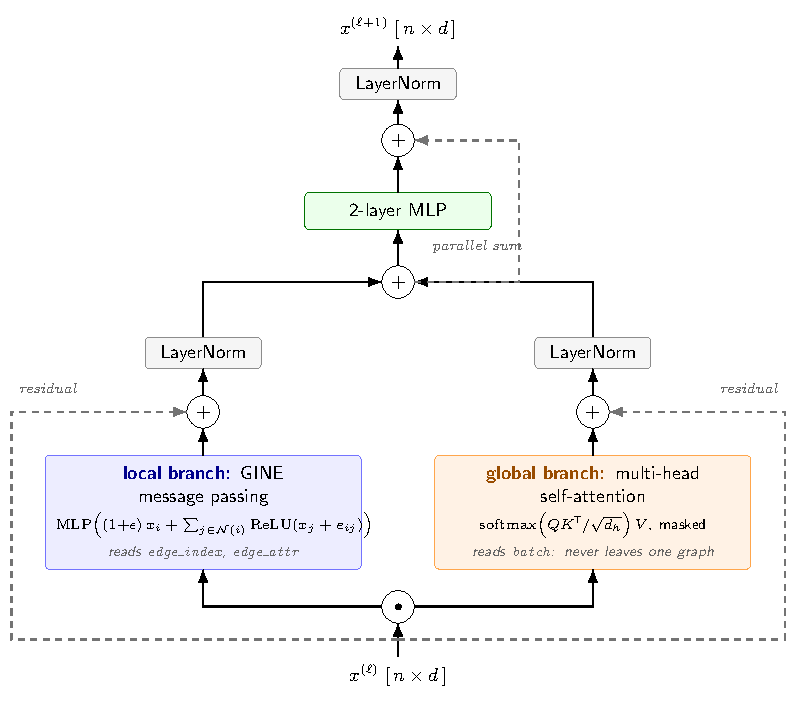
\includegraphics[width=0.78\linewidth]{fig_p2_layer.pdf}
  \caption{One \texttt{HybridGTLayer}. Both branches read $x^{(\ell)}$; dashed arrows are
           residual connections.}
  \label{p2:fig:layer}
\end{figure}

\subsection*{Implementation}

\lstdefinestyle{p2python}{%
  language=Python, basicstyle=\footnotesize\ttfamily,
  keywordstyle=\color{blue!55!black}, commentstyle=\itshape\color{black!55},
  stringstyle=\color{green!35!black}, showstringspaces=false,
  breaklines=true, breakatwhitespace=true, keepspaces=true,
  frame=single, rulecolor=\color{black!30}, framerule=0.3pt,
  xleftmargin=4pt, xrightmargin=2pt, aboveskip=8pt, belowskip=4pt,
}

\noindent\texttt{HybridGT} (cell~22) is used unchanged.

\begin{lstlisting}[style=p2python]
class HybridGTLayer(nn.Module):
    """One GraphGPS-style hybrid layer: a local message-passing branch and a
    global self-attention branch, run in parallel on the same input and summed.
    """

    def __init__(self, dim, heads, num_bond_types=4):
        super().__init__()
        self.dim, self.heads = dim, heads
        # local branch: GINE message passing
        self.bond = nn.Embedding(num_bond_types, dim)
        self.eps = nn.Parameter(torch.zeros(1))
        self.mpnn = nn.Sequential(nn.Linear(dim, 2 * dim), nn.ReLU(),
                                  nn.Linear(2 * dim, dim))
        # global branch: multi-head self attention inside each graph
        self.qkv = nn.Linear(dim, 3 * dim)
        self.proj = nn.Linear(dim, dim)
        # fusion
        self.norm_local = nn.LayerNorm(dim)
        self.norm_global = nn.LayerNorm(dim)
        self.ffn = nn.Sequential(nn.Linear(dim, 2 * dim), nn.ReLU(),
                                 nn.Linear(2 * dim, dim))
        self.norm_ffn = nn.LayerNorm(dim)

    def local_branch(self, x, edge_index, edge_attr):
        """GINE: every message carries its bond type, neighbours are summed."""
        src, dst = edge_index
        msg = F.relu(x[src] + self.bond(edge_attr))        # [E, dim]
        agg = torch.zeros_like(x).index_add_(0, dst, msg)  # [num_nodes, dim]
        return self.mpnn((1 + self.eps) * x + agg)

    def global_branch(self, x, batch):
        """Self attention; the padding mask keeps it inside a single graph."""
        h, mask = to_dense_batch(x, batch)          # [B, N, dim], [B, N]
        B, N, D = h.shape
        qkv = self.qkv(h).view(B, N, 3, self.heads, D // self.heads)
        q, k, v = qkv.permute(2, 0, 3, 1, 4)        # each [B, heads, N, D/heads]
        scores = q @ k.transpose(-1, -2) / math.sqrt(D // self.heads)
        scores = scores.masked_fill(~mask[:, None, None, :], float("-inf"))
        weights = torch.softmax(scores, dim=-1).nan_to_num(0.0)
        out = (weights @ v).transpose(1, 2).reshape(B, N, D)
        return self.proj(out)[mask]                 # back to [num_nodes, dim]

    def forward(self, x, edge_index, edge_attr, batch):
        """x          : [num_nodes, dim], node states of the whole batch
        edge_index : [2, E]
        edge_attr  : [E], bond type ids in [0, 4)
        batch      : [num_nodes], graph id of every node
        Returns new node states [num_nodes, dim]."""
        local = self.local_branch(x, edge_index, edge_attr)
        glob = self.global_branch(x, batch)
        h = self.norm_local(x + local) + self.norm_global(x + glob)
        return self.norm_ffn(h + self.ffn(h))
\end{lstlisting}

\subsection*{Results}

\begin{table}[H]
  \centering
  \small
  \caption{ZINC, 30 epochs; lower MAE is better, and the epoch is selected on validation
           MAE. Each row is the mean over independent runs at different seeds, with their
           standard deviation. Repeating a single configuration unchanged already moves test
           MAE by a comparable amount on this CPU, so the sd is a run-to-run noise floor
           rather than a seed effect alone. ``params'' counts only parameters that receive a
           gradient, so an ablation is not credited with the branch it never calls. The
           bold row is the submitted layer, not the best number in the column.}
  \label{p2:tab:zinc}
  \begin{tabular}{lrrrrrr}
    \toprule
    & \multicolumn{2}{c}{val MAE} & \multicolumn{2}{c}{test MAE} & & \\
    \cmidrule(lr){2-3}\cmidrule(lr){4-5}
    model & mean & sd & mean & sd & params & runs \\
    \midrule
    plain graph transformer (no structural information) & 0.649 & 0.004 & 0.693 & 0.002 & 139.6k & 3 \\
    demo: degree centrality + common-neighbour bias & 0.469 & 0.015 & 0.495 & 0.018 & 143.9k & 3 \\
    \midrule
    \textbf{hybrid GT (cell 22): parallel sum} & 0.350 & 0.007 & 0.364 & 0.008 & 211.6k & 6 \\
    \quad ablation: global branch removed & 0.353 & 0.008 & 0.367 & 0.007 & 144.5k & 6 \\
    \quad ablation: local branch removed & 0.533 & 0.003 & 0.573 & 0.003 & 143.7k & 3 \\
    \midrule
    \quad instead: attention reads the MPNN output & 0.347 & 0.006 & 0.359 & 0.007 & 211.6k & 6 \\
    \quad instead: a learned gate in place of the sum & 0.340 & 0.009 & 0.355 & 0.005 & 244.6k & 6 \\
    \bottomrule
  \end{tabular}
\end{table}

The hybrid cuts the plain transformer's test MAE from 0.693 to 0.364 and beats the
demo encoding at 0.495. The ablation says which branch does it: removing attention
changes nothing beyond run-to-run noise (0.367), removing message passing costs
0.573. Repeating one configuration unchanged already moves test MAE by 0.009 here,
the bar the rest has to clear. Every hybrid run peaks in the final three epochs, so 30 stops
it early, and at 100 (one run each) the gap opens the other way --- local only 0.251 against 0.283. Stacking the branches matches summing them (0.359), and the gate is
the best of the three at 0.355 --- by about one noise width, and with 16\% more
parameters, so I kept the plain sum.

The global branch is not short of range: ZINC molecules have mean diameter $12.5$, and four
message-passing rounds cover only $51.8\%$ of node pairs. It is short of \emph{identity}.
Degree centrality --- the absolute encoding \texttt{HybridGT} fixes --- takes four values and
gives half of all atoms the same one, so attention can average over a molecule but hardly
tell which atom it reads. Of GraphGPS's three ingredients, the one missing here is the first,
the positional/structural encoding.

